\documentclass[a4paper, openright, 12pt]{report}
\usepackage[spanish,es-tabla]{babel}
\usepackage[spanish]{babel}
\usepackage[utf8]{inputenc}
\usepackage[final]{graphicx}
\usepackage{url}
\usepackage{hyperref}
\usepackage{enumerate}
\usepackage{graphicx}
\usepackage{subfiles}
\usepackage{blindtext}
\usepackage{amsmath}
\usepackage{float}
\usepackage{sidecap}
\usepackage{algpseudocode}
\usepackage{subcaption}
\usepackage{listings}
\usepackage{color}
\usepackage{wrapfig}
\usepackage{datetime}
\usepackage[none]{hyphenat}
\usepackage{setspace} 
\usepackage{epstopdf} %converting to PDF 
\setboolean{@twoside}{false}  %For add pdf page
\usepackage[final]{pdfpages}  %For add pdf page


\graphicspath{ {../imgs/} {../../imgs/} }
\sloppy
\spacing{1.25} 

\definecolor{codegreen}{rgb}{0,0.6,0}
\definecolor{codegray}{rgb}{0.5,0.5,0.5}
\definecolor{codepurple}{rgb}{0.58,0,0.82}
\definecolor{backcolour}{rgb}{0.95,0.95,0.92}
 
\lstdefinestyle{mystyle}{
    backgroundcolor=\color{backcolour},   
    commentstyle=\color{codegreen},
    keywordstyle=\color{magenta},
    numberstyle=\tiny\color{codegray},
    stringstyle=\color{codepurple},
    basicstyle=\scriptsize,
    breakatwhitespace=false,         
    breaklines=true,                 
    captionpos=b,                    
    keepspaces=true,                 
    numbers=left,                    
    numbersep=5pt,                  
    showspaces=false,                
    showstringspaces=false,
    showtabs=false,                  
    tabsize=2
}
 
\lstset{style=mystyle}

\begin{document}

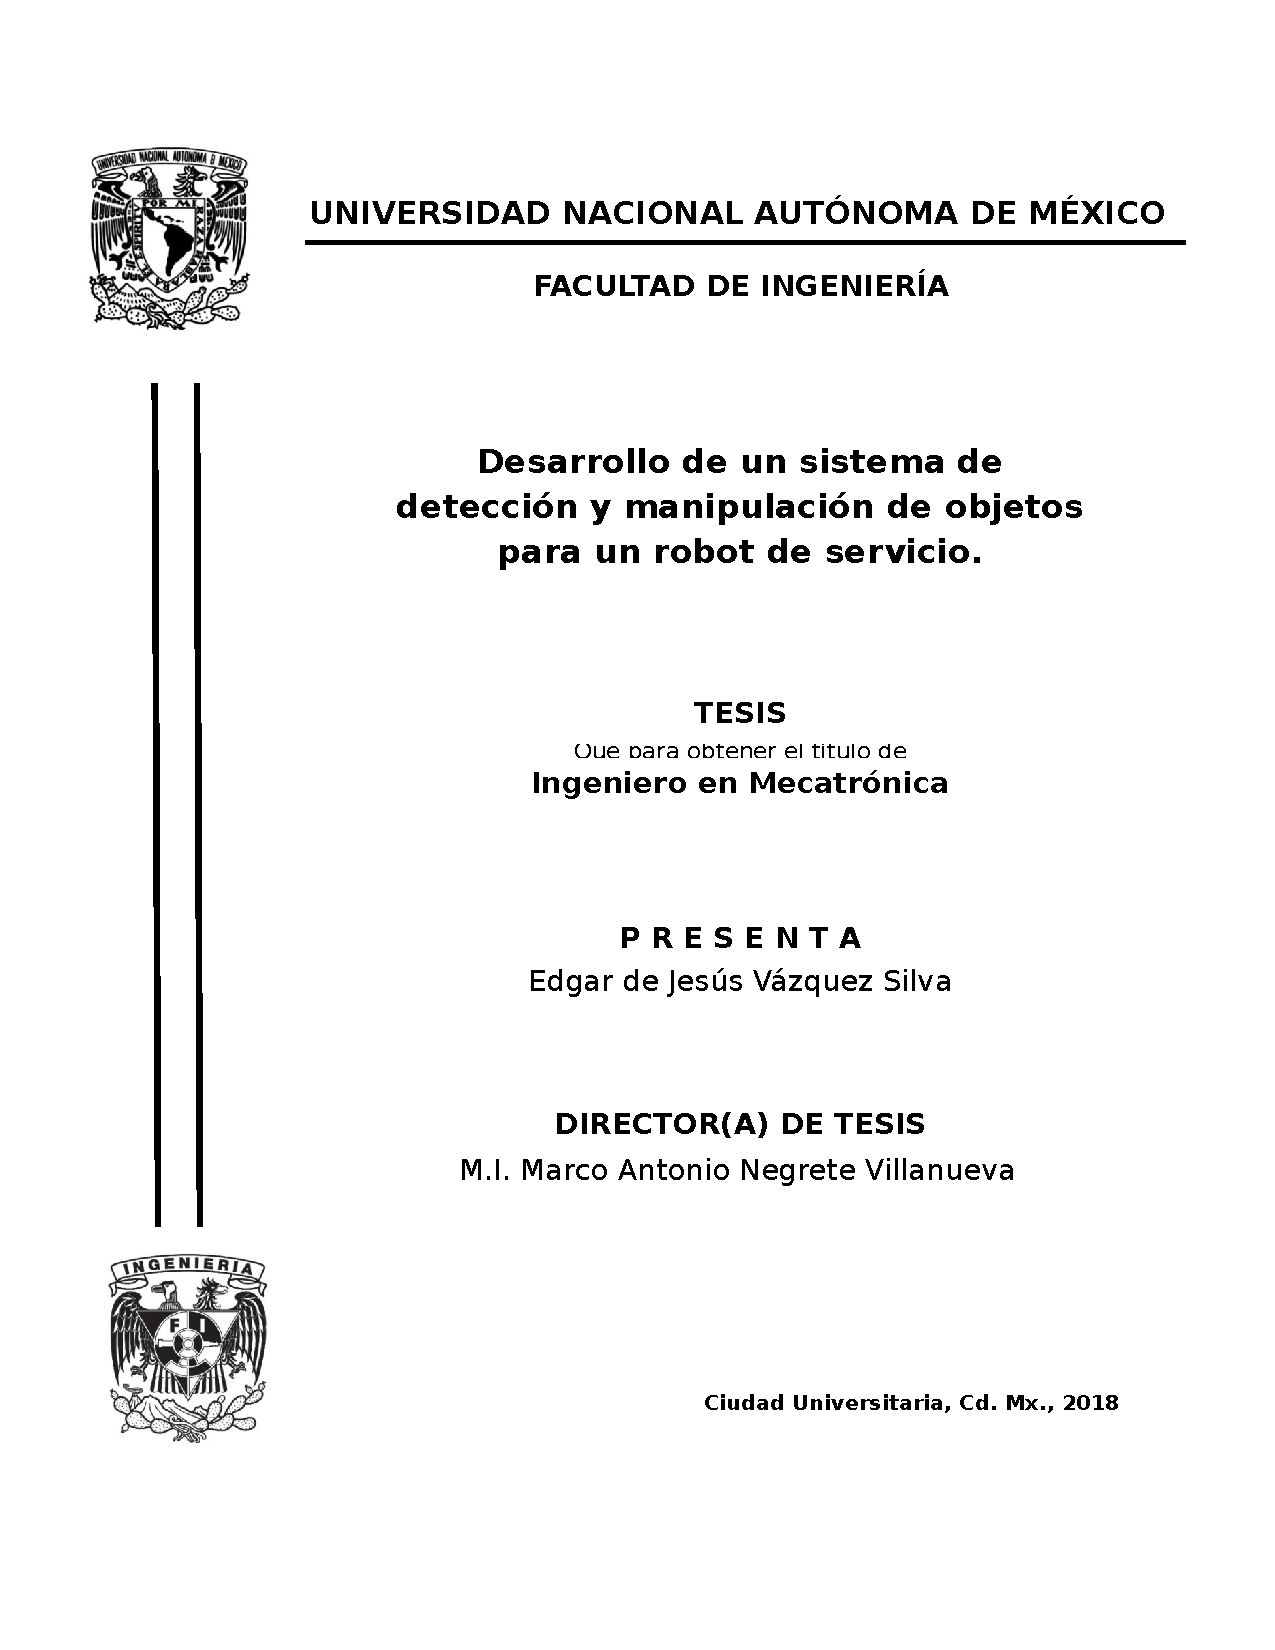
\includepdf[pages=-]{../pdf/portada.pdf}

% \begin{titlepage}
% 	\begin{center}
% 		\vspace*{-1in}
% 		\begin{figure}[htb]
% 			\begin{center}
% 			
\includegraphics[width=3.5cm, height=4cm]{/unam.png}
% 			\end{center}
% 		\end{figure}
% 		\vspace*{0.35in}

% 		\begin{large}
% 			\rule{130mm}{0.1mm}\\
% 			UNIVERSIDAD NACIONAL AUTÓNOMA DE MÉXICO
% 		\end{large}
% 		\vspace*{0.55in}

% 		FACULTAD DE INGENIERÍA \\
% 		\vspace*{0.25in}
% 		DEPARTAMENTO DE INGENIERÍA MECÁNICA E INDUSTRIAL\\
% 		\vspace*{0.6in}
% 		\begin{large}
% 			TESIS:\\
% 		\end{large}
% 		\vspace*{0.2in}

% 		\begin{Large}
% 			\textbf{ Desarrollo de un sistema de detección y manipulación de objetos para un robot de Servicio} \\
% 		\end{Large}
% 		\vspace*{0.65in}

% 		\rule{110mm}{0.1mm}

% 		\vspace*{0.35in}
% 		\begin{large}
% 			Edgar de Jesús Vázquez Silva \\
% 			\vspace*{0.55in}
% 			\today
% 		\end{large}


% 	\end{center}
% \end{titlepage}



\tableofcontents{}


\newpage{}

\subfile{sections/01_introduccion}

\subfile{sections/02_marcoTeorico}

\subfile{sections/03_deteccionObjetos}

\subfile{sections/04_manipulador}

\subfile{sections/05_integracion}

\subfile{sections/06_resultadosConclusiones}

\newpage{}


\bibliographystyle{ieeetr}
\bibliography{biblio.bib}



\end{document}

